% Appendix: Procedure to download the application
\chapter{Procedure to Install the Application for Testing}
\label{app:download}
\clearpage

Android and iOS testers install SanCarGo in different ways (Section~\ref{sec:install}).

\section*{L.1 Android: Firebase App Distribution (UAT)}
Figure~\ref{fig:download} shows the steps that every Android tester follows, from the invitation email to the first launch of the application. An invitation is valid for 30 days.

\begin{figure}[htbp]
    \centering
    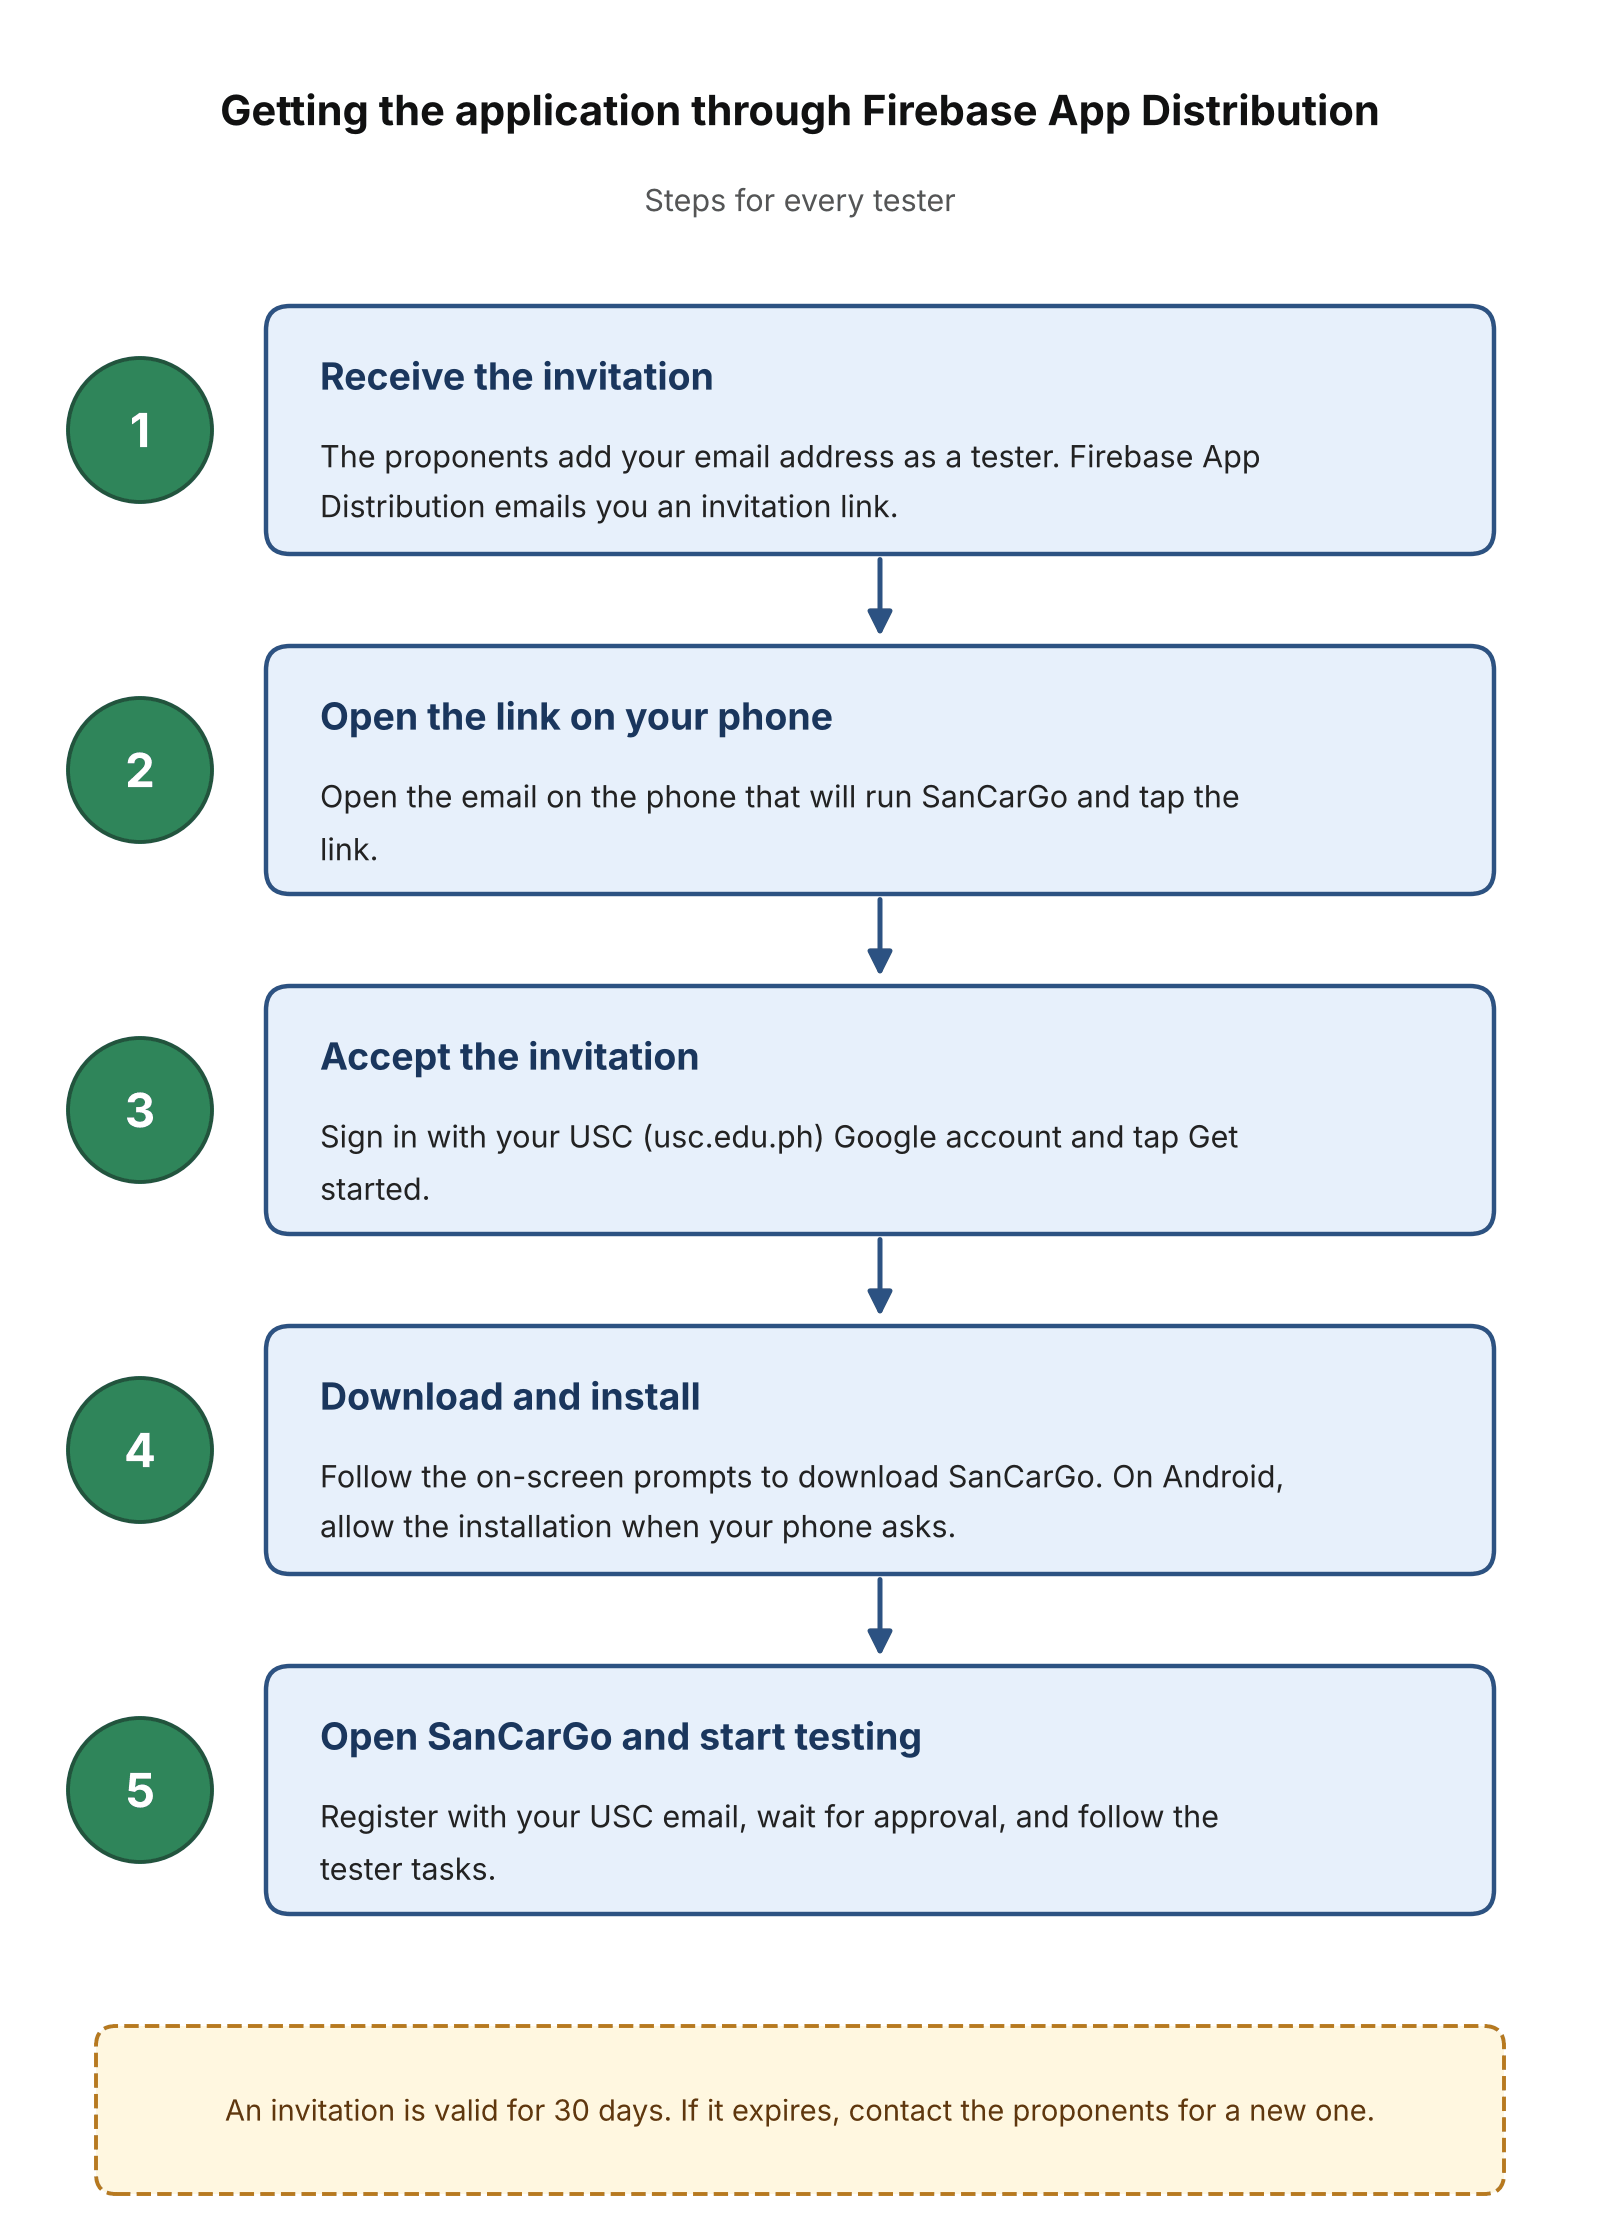
\includegraphics[width=0.78\textwidth,height=0.78\textheight,keepaspectratio]{images/app_distribution_steps.png}
    \caption{Steps to download SanCarGo through Firebase App Distribution (Android)}
    \label{fig:download}
\end{figure}

\clearpage
\section*{L.2 iOS: Installation from Xcode (alpha, beta, and UAT)}
The same steps were used for alpha testing, beta testing, and UAT onboarding. In alpha and beta testing, the proponents signed in with their own Apple IDs. In UAT onboarding, each participant signed in with his or her own Apple ID in Xcode on the proponents' computer.
\begin{enumerate}
    \item Sign in with an Apple ID in Xcode.
    \item Create a Bundle Identifier for that Apple ID in Firebase and set it up in the Google Cloud Console. A new Bundle Identifier is made for each Apple ID.
    \item Download the GoogleService-Info.plist file of the Bundle Identifier from Firebase and configure it in Xcode.
    \item In Xcode, under Signing \& Capabilities, select the Apple ID under Team and enter the Bundle Identifier.
    \item Plug in the iOS device and enable Developer Mode on it.
    \item After the device restarts, build the application onto it.
    \item On the device, trust the Apple ID under General, VPN \& Device Management in the Settings application.
    \item Open the SanCarGo application.
\end{enumerate}
Because free Apple ID accounts were used, the installed application stops opening after seven days, so it was reinstalled on each iOS device after seven days.
